\section{The \GP Variable-Pitch IFU}
\label{sec:pak}

\subsection{Design}
\label{sec:GP_design}

\begin{figure*}[t]
  \centering
\vskip -0.65in
  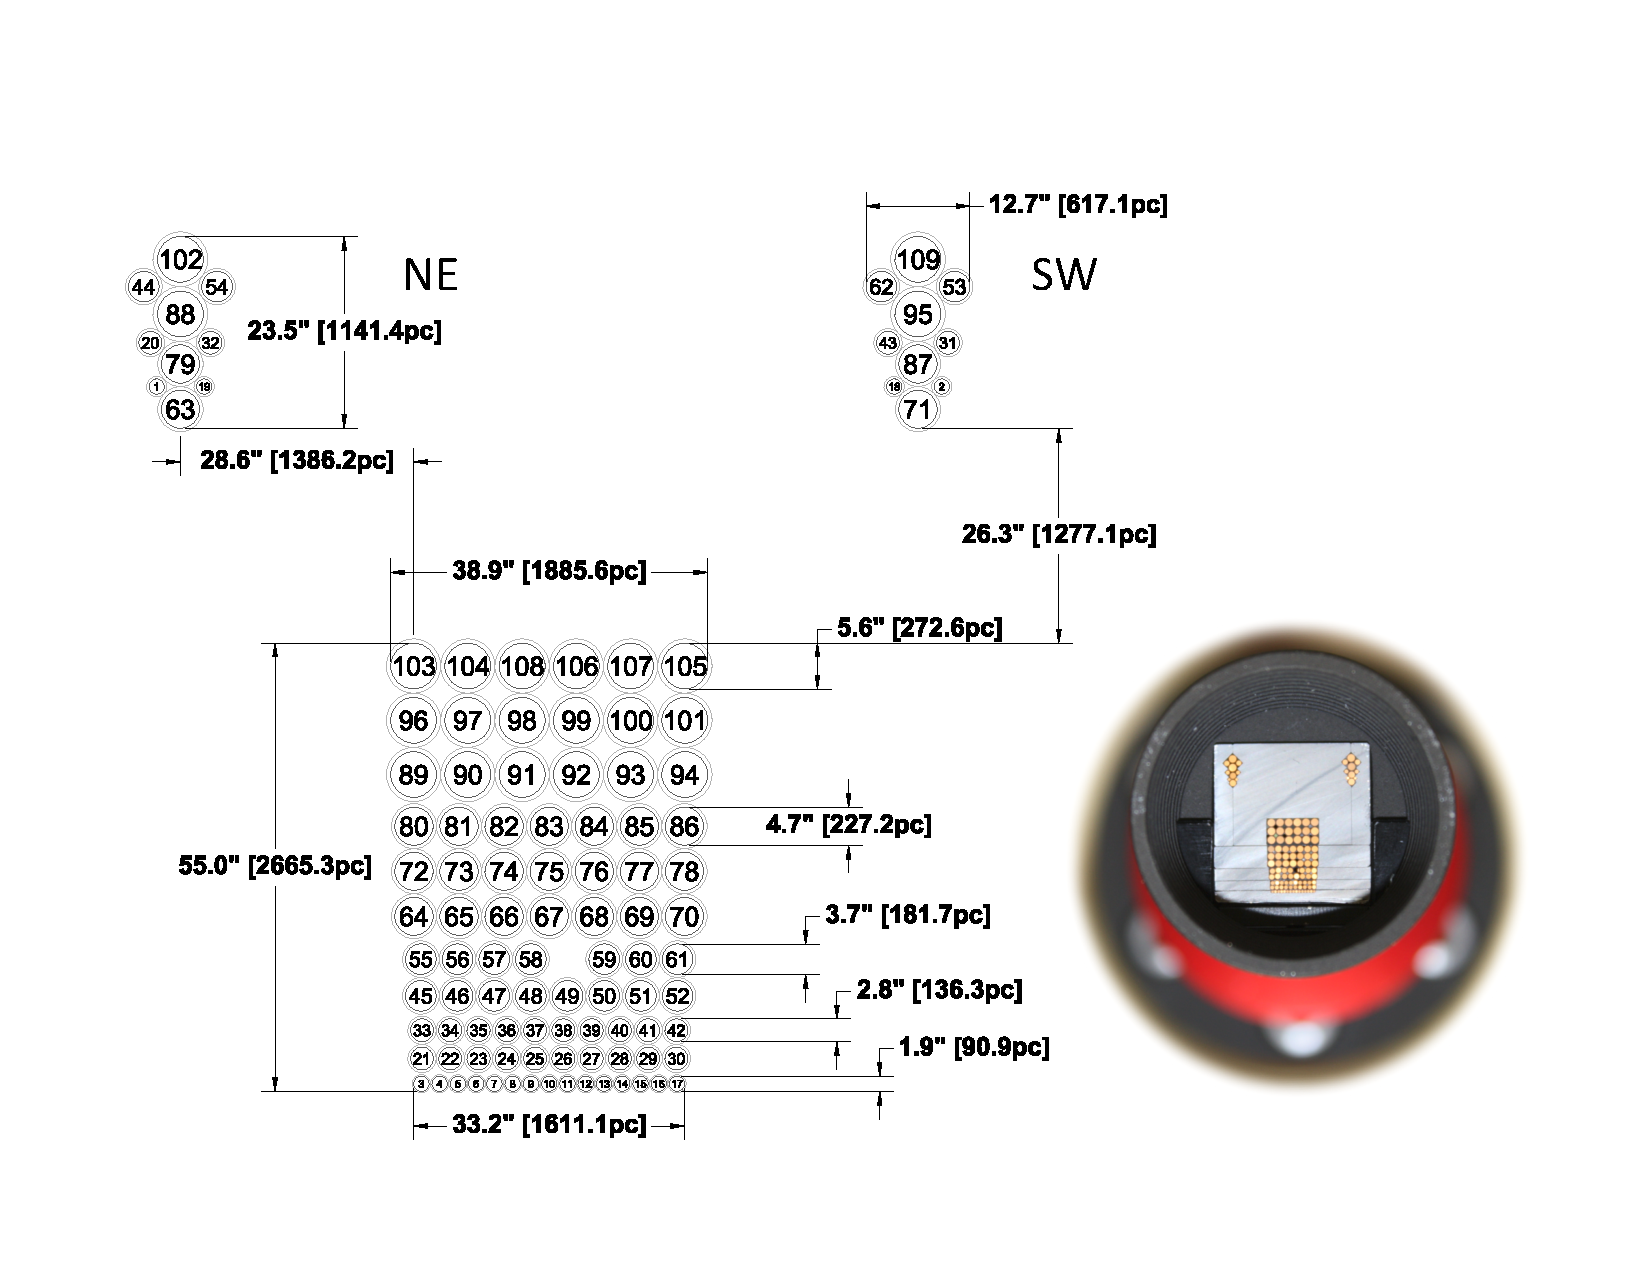
\includegraphics[width=\textwidth]{891_1/figs/GradPak_labeled_inset_ALT.pdf}
\vskip -0.35in
  \caption{\label{fig:GradPak}\GP IFU on the WIYN 3.5m
    Telescope. Distances are in arcseconds and in kpc for a distance
    of 10 Mpc. The inset image shows the completed IFU in its mounting
    bracket. Note aluminum fixture and absence of packing fibers.}
\end{figure*}

The \GP integral field unit (IFU) is mounted on the WIYN\footnote{The
  WIYN Observatory is a join facility of the University of
  Wisconsin-Madison, Indiana University, NASA, and the National
  Optical Astronomy Observatory.}  Bench Spectrograph
\citep{Barden94,Bershady08,Knezek10} and makes up one half of the
novel HexPak/\GP IFU system \citep{Wood12}, a pair of IFUs that have
unique fiber configurations and share a common slit. The fiber
geometry of \GP is optimized for observations of edge-on galaxies;
five different fiber sizes are arranged in a rectangular gradient
pattern that allows for efficient observations of objects with
significant surface brightness gradients on scales of roughly an
arcminute (Figure \ref{fig:GradPak}).  A list of fiber diameters can
be found in Table \ref{tab:GradPak}. The increase in fiber size across
the array corresponds to equal signal-to-noise (S/N) per unit
wavelength in the source or background-limit for light distributions
with e-folding scales of 26 to 50 arcsec. This corresponds to vertical
scale-heights of 1.3 to 2.4 kpc at a distance of 10 Mpc, comparable to
the thickest possible disk components in NGC 891.  In practice, the
complex vertical structure of stars and dust in galaxy disks such NGC
891's make the S/N optimization imperfect. This instrument design, by
attempting to achieve similar signal-to-noise per exposure in all
fibers, maximizes mapping efficiency at the cost of reduced spatial
and spectral resolution in the larger fibers at larger
scale-heights. This trade-off is sensible given the increased
e-folding scale of the disk away from the mid-plane, and the
commensurate expectation of large velocity dispersions.

The physical layout of \GP consists of a main array and two groups of
offset sky fibers. The main array is a 55 arcsec high stack of pseudo
slits with increasing slit-width and fiber diameters (Figure
\ref{fig:GradPak}). The fibers used are broad spectrum, stepped index,
fused silica fibers (Polymicro FBP) with core diameters between
\val{200}{\mu m} and \val{600}{\mu m} (corresponding to \val{1.87}{''}
to \val{5.62}{''} at the WIYN f/6.3 focal plane). The non-active
(i.e., cladding and buffer) portion of each fiber takes up an
additional 20\% of each fiber's physical diameter. The pseudo-slits
are grouped into blocks that contain all the fibers of the same
size. The blocks were assembled sequentially from small to large fiber
sizes to build up the entire stack. Each block is mechanically bounded
by precision layers of aluminum, located with pins. The smallest
fibers have only one row (or pseudo-slit) that is 33.2 arcsec in
length; the two largest fibers sizes have three rows each, with a
maximum pseudo-slit length of 38.9 arcsec; while the intermediate
sizes have two rows. After a block has been assembled, glued and
cured, it is separated from the next block by a plastic shim that is
\val{25.4}{\mu m} (\val{0.24}{''}) thick; this separation is a key
component of the assembly and curing process.  While the scientific
design of \GP required a non-optimal fiber packing arrangement, the
total packing efficiency (defined as light-gathering area divided by
total area) of the main array is roughly 55\%.

The sky fibers of \GP occupy two sub arrays that are offset
\val{26.3}{''} vertically and \val{28.6}{''} horizontally on either
side of the main array. On NGC 891 this places the sky fibers
\val{1.3}{kpc} above the top of \GP and \val{\sim 3.8}{kpc} from the
plane of the galaxy, far above measurable flux from the galaxy
\citep{Rand11}. The sky fibers were assembled separately in machined
blocks that are mechanically attached to the main array. This assembly
was polished as a single, assembled unit. The polishing process was
similar to what was undertaken for SparsePak \citep{Bershady04}.

\GP does not have any packing fibers. Instead, the physical layout is
established with a custom-built aluminum fixture, as described above
and in \citep{Wood12}. Based on the results of
\S\ref{sec:gradpak_performance} we do not think the lack of buffering
fibers causes a significant loss of performance. However, the use of
aluminum, and in particular the aluminum shim material comprising the
walls of the pseudo-slit layers is not optimal for optical polishing,
with deleterious effects noted in \S\ref{sec:gradpak_performance}. A
lesson learned is that the fabrication ease, efficiency and low
machining cost of aluminum does not out-weigh the superior performance
of suitable stainless steel, invar or ceramics, which we would
recommend for future builds. In contrast, for example, the stainless
steel ferrules used in MaNGA in SDSS-IV provided outstanding fixturing
for obtaining good optical finish on the polished fibers (Drory et
al. 2014).  We note that the challenges with the aluminum fixture for
\GP is was not an issues for HexPak which, like its predecessors
DensePak (Barden et al. TODO) and SparsePak (Bershady et al. 2004)
consisted of an entirely fused-silica array.

Further details of the design and construction of HexPak/\GP,
including cable design, fabrication and commercial product
descriptions for specific components can be found in \citet{Wood12}.
Notable are the dual-slit assembly that sits inside a standard Bench
Spectrograph fiber ``foot,'' as well as the rotation couplers that
ease handling will minimizing stress-inducing torsion on the fibers
during telescope rotator motion.

\begin{deluxetable}{ccccc}
\tablewidth{0pt}
\tablecaption{\GP Fiber Diameters}
\tablehead{
  & 
  \colhead{spatial} &
  \colhead{spectral\,\tablenotemark{a}} &
  &  \\
  \colhead{($\mu$m)} &
  \colhead{(pixels)} &
  \colhead{(pixels)} &
  \colhead{(arcsec)} &
  \colhead{(pc\,\tablenotemark{b})}
}
\startdata
200 & 4.64 & 4.36 & 1.87 & 90.9\\
300 & 6.96 & 6.55 & 2.81 & 136\\
400 & 9.28 & 8.73 & 3.75 & 182\\
500 & 11.6 & 10.9 & 4.69 & 227\\
600 & 13.9 & 13.1 & 5.62 & 273
\enddata
\label{tab:GradPak}
\tablenotetext{a}{Assuming the anamorphic factor in Table \ref{tab:spec}}
\tablenotetext{b}{Assuming a distance of \val{10}{Mpc} to NGC 891.}
\end{deluxetable}

\subsection{Mechanical Performance}

Despite best effort and extensive testing to develop best practices,
the mechanical alignment of the \GP fibers has some noticeable
imperfections. In Appendix \ref{sec:GPtesting} we provide a
high-resolution image (Figure \ref{fig:gradpak_face}) of the as-built
fiber array to document this. The irregularities are particularly
notable for the 400 $\mu$m (3.75 arcsec) fiber pseudo-slits for which
some fibers have offsets from their idealized location (Figure
\ref{fig:GradPak}) by as much as 0.5 arcsec. The other pseudo-slits
have internal and relative alignment to other pseudo-slits that we
estimate are accurate at the 0.l-0.2 arcsec level. Table
\ref{tab:GP_cal} in the Appendix provides the
idealized fiber locations corresponding to Figure
\ref{fig:GradPak}. These should suffice for almost all applications
except the most demanding that for whatever reason require very high
precision relative astrometry. Should the need arise, Figure
\ref{fig:gradpak_face} will be made available upon request. Overall,
the final IFU has good-to-excellent mechanical regularity.

\subsection{Optical Performance}

\label{sec:gradpak_performance}

The IFU face and slit were both polished to a \val{0.5}{\mu m} grit
level to mitigate throughput losses caused by surface scattering
\citep{Eigenbrot12}. Material from the aluminum fixture was seen to
form deposits on the fiber faces, with some performance degradation
that we summarize here and detail in Appendix \ref{sec:GPtesting}.

Laboratory measurements of throughput and focal-ratio degradation
(FRD) in the Johnson $V$ revealed distinct performance gradients
across the array. Some of the throughput variations are likely due to
polish imperfections from aluminum residue. However, we find FRD
systematically decreases with larger fiber size, with a small upturn
for the largest fibers. Unfortunately we cannot separate systematic
performance differences for different fiber core sizes from
differences in handling and assembly process. We also find, not
surprisingly, that FRD correlates to first order with throughput, but
that there is a bimodal distribution in transmission and FRD which
indicates several processes at work in determining fiber performance.

Overall, the throughput defined for $f$/6.3 fiber input from the
telescope and the $f$/4 out speed matching the Bench Spectrograph
collimator has a maximum of 90\% and a minimum of 50\% at 550 nm. The
mean throughput for all fibers is 80\%, with means by fiber size of
70, 81,84, 83, 79\%, from small to large. Means for sky fibers are
comparable, within a percent. We compared our lab measurements to the
relative throughput from dome-flats measurements once \GP was
installed on the telescope. This comparison shows that the
on-telescope {\it relative} performance is the same, indicating
throughput variations are intrinsic to the cable and not the
spectrograph, consistent with expectations for the performance of the
upgraded Bench Spectrograph \citep{Bershady08,Knezek10}.

One of the 3.75'' fibers (between fibers 58 and 59 as marked in Figure
\ref{fig:GradPak}) fractured during polishing. The fracture is close
to the surface and likely could be polished out; this was deemed
impractical to pursue due to the indeterminate fracture depth and the
risk of exceeding the finite gluing length. The fracture leaves 10\%
of the fiber face intact and transmitting, but for practical purposes
this fiber is considered not usable and ignored in all astrometry
tables.  A close-up image of the \GP fibers that shows polishing
imperfections and the broken fiber can be found in Figure
\ref{fig:gradpak_face}.  Despite these imperfections, the final IFU
has good transmission performance.

\subsection{Installation}
\label{sec:install}

Final construction of \GP was completed in September 2013.  HexPak/\GP
were then installed at WIYN during November 2013. The 25 m of cabling
that contain the IFUs are routed from the Bench Spectrograph room, up
through the central bearing of the azimuth drive, out of one of the
telescope forks, and onto a tray designed to hold the SparsePak
cable. During observations one of the IFU heads is plugged into the
the WIFOE\footnote{WIYN Indiana Fiber Optic Echelle} port, which
provides common IFU access to the IAS\footnote{Imaging Acquisition
  System} on one of WIYN's nasymth ports. During cable routing a
section of cabling developed a hole that was the result of bend stress
causing the helical wrapping of the cable to come undone. This hole
was repaired on site and is located just within the fork on the
observing floor. Fibers were not damaged, and the cable integrity has
been deemed acceptable for the life of \GP.

During installation we confirmed that both the HexPak and \GP slits
occupy the same focal plane, which allows the heads to be switched at
the telescope end without the need to adjust the Bench Spectrograph.
We also adjusted the precise location of the HexPak, \GP, and
SparsePak \citep{Bershady05} fiber faces so that they share a common
focus in the port. The common focus locations at both ends of the
fiber cable allow users to switch between HexPak and \GP in only a few
minutes during the night, which allows great flexibility in scheduling
multiple programs on the same night.

In addition to access for the WIYN IFUs the WIFOE port has a pellicle
and camera that allow observers to see an image of the IFU fibers
overlaid on the view from the telescope focus. To resolve the smallest
fibers in HexPak/\GP the existing WIFOE camera was replaced with an
Allied GigE GT3300 CCD with a default resolution of
0.258''/pixel\footnote{more information can be found at
  \url{http://www.wiyn.org/Instruments/WifoeCameraInterface.pdf}}.
